\documentclass{article}
\usepackage[utf8]{inputenc}
\usepackage{amsmath}
\usepackage{graphicx}

\title{Assignment 6}
\author{Swapnil Sirsat }
\date{January 2021}

\begin{document}

\maketitle

\section*{Question}
Can you construct a rhombus ABCD with
AC = 6 and BD = 7?
\section*{Answer}
assuming that the diagonals intersect at (0,0) \\
and we know that the diagonals bisect each other at 90$^\circ$
The four vertices of the diagonals can be easily calculated\\
\begin{gather*}
    AC = 6
\end{gather*}
and taking the diagonal AC has a slope of 1 \\
Equation for line AC becomes\\
\begin{gather*}
    x = y
\end{gather*}
therefore the points A and C become
\begin{gather*}
    A = (-3,-3)\\
    C = (3,3)
\end{gather*}
now, since the diagonals bisect each other at 90$^\circ$
slope of BD becomes -1 and since the diagonals are passing through (0,0)
Equation of BD becomes 
\begin{gather*}
    x = -y
\end{gather*}
hence, the point B and D are
\begin{gather*}
    B = (3.5,-3.5)\\
    D = (-3.5,3.5)
\end{gather*}
\newpage
now joining these points we get the rhombus ABCD
\\ which is shown in below figure

\begin{figure}[h!]
    \centering
    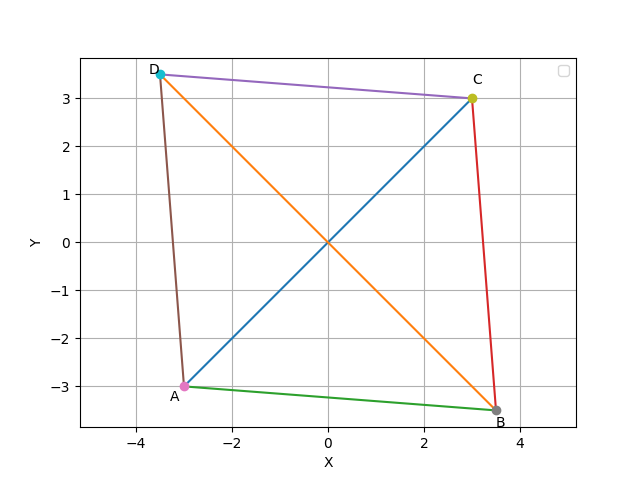
\includegraphics{Figure_1.png}
    \caption{Rhombus ABCD}
    \label{fig:my_label}
\end{figure}
\newpage
\section*{Quesiton}
Draw a circle of diameter 6.1
\section*{Answer}
since the diameter = 6.1\\
radius of the circle is 
\begin{gather*}
    r = 6.1/2
\end{gather*}
Taking the center at 
\begin{gather*}
    O(0,0)
\end{gather*}
we can draw the circle
the output figure is as below
\begin{figure}[h!]
    \centering
    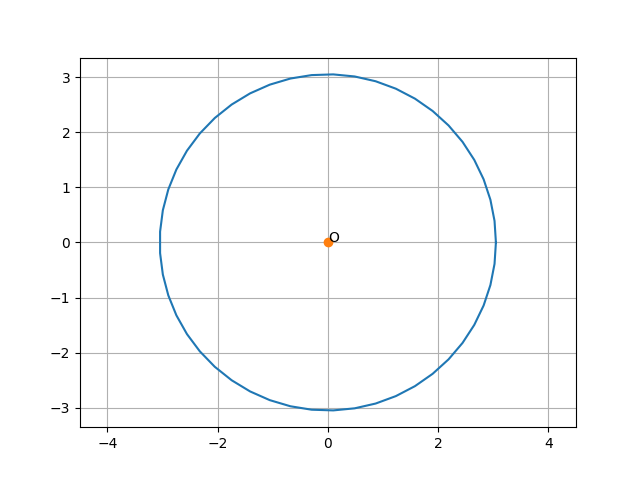
\includegraphics[height = 300]{Figure_2.png}
    \caption{Circle O}
    \label{fig:my_label}
\end{figure}

\end{document}
